\section{What the Smooth Flow Buys and What It Costs}
\label{sec:buys-costs}

\paragraph{Anytime reading with the frozen decoder.}
After a prefix of stage~3 we skip the rest of the stage and classify with the model's
own trained downsample, stage~4 and head (\cref{fig:prefix-acc,fig:block-evals}; full
validation).
No probe is trained~\citep{alain2016probes,belrose2023tuned}, so the score measures how
close each prefix is to the state the decoder expects.
On native prefixes, top-1 at $t{=}3$ is $\prefixTiedThree\%$ for the tied stage against
$\prefixUntiedThree\%$ for the untied one; at $t{=}5$ it is $\prefixTiedFive\%$ against
$\prefixUntiedFive\%$.
Refining the path at $R{=}20$ moves the same curves only slightly
($\prefixTiedThreeR\%$ and $\prefixUntiedThreeR\%$ at $t{=}3$).
The decoder was trained on $x_T$, so a low score does not mean that early features lack
information; it means that the tied state enters the decoder's operating region earlier,
as the alignment and $t_{50}$ of \cref{sec:nine-directions} suggest.
Alignment and $t_{50}$ are consistent with this mechanism; they do not prove it
causally.
The frozen decoder is the right measure of early exit without training extra heads: the
tied stage is anytime with its own downstream network.

\begin{figure}[t]
    \centering
    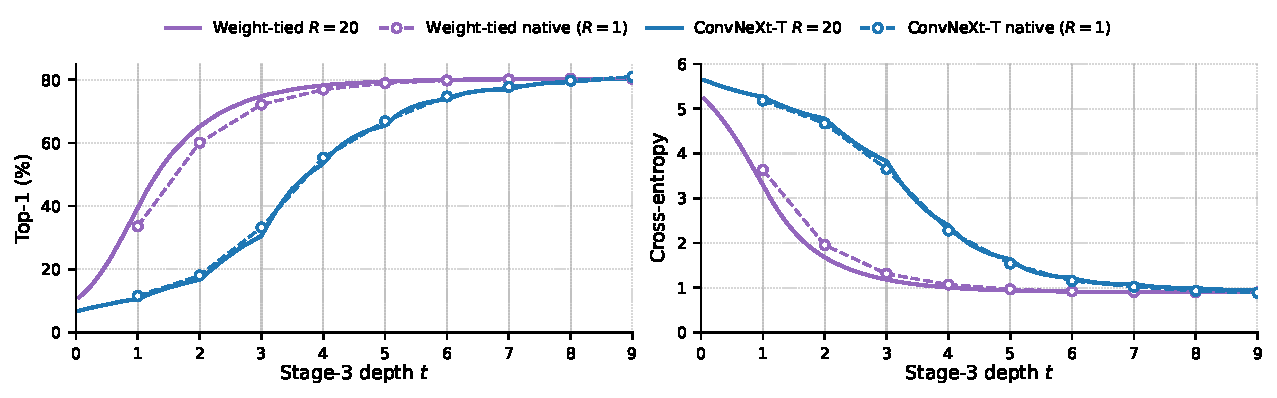
\includegraphics[width=\linewidth]{figures/prefix_s4_head_acc.pdf}
    \caption{Top-1 (left) and cross-entropy (right) of each model's frozen stage~4 and
    head on stage-3 prefixes (full validation).
    Solid: refined path ($R{=}20$, $\Delta t{=}0.05$); open markers: native prefixes
    at block ends.
    The tied stage is readable much earlier; a low early score does not imply that early
    features lack information.}
    \label{fig:prefix-acc}
\end{figure}

\begin{figure}[t]
    \centering
    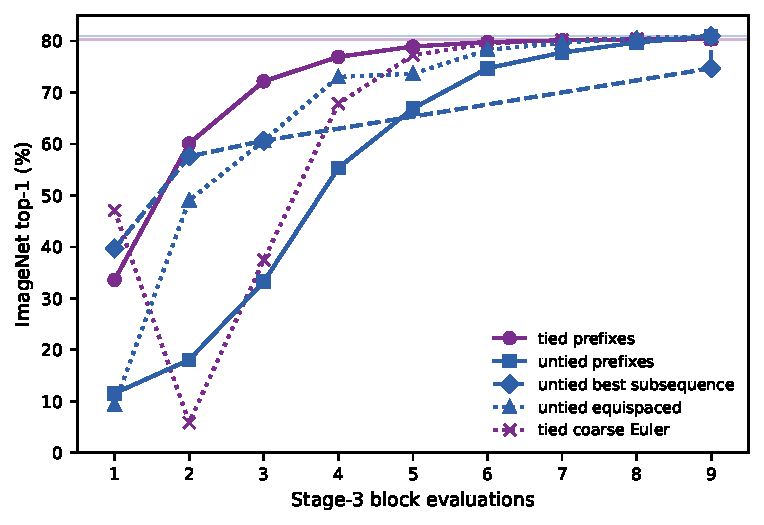
\includegraphics[width=\linewidth]{figures/block_evals_acc.pdf}
    \caption{ImageNet top-1 against the number of stage-3 block evaluations (Euler
    counts $1$ per step), without retraining.
    Purple solid: native tied prefixes ($k{=}1{\ldots}9$).
    Blue solid: native untied prefixes.
    Blue dashed: selected untied subsequences from App.~\ref{app:block-ops}.
    Blue dotted: equispaced untied subsets
    $\mathrm{round}(\mathrm{linspace}(0,8,L))$ with $\Delta t{=}9/L$
    (\cref{tab:app-equispaced}).
    Purple dotted: coarse Euler of the tied stage at $T{=}9$
    (App.~\ref{app:solvers}).
    Horizontal lines: full-depth accuracy of each model.
    The tied stage dominates at few evaluations through its prefixes; the untied stage
    wins at nine; coarse Euler of the tied stage is not the way to save compute.}
    \label{fig:block-evals}
\end{figure}

\Cref{fig:block-evals} puts the same prefixes on a compute axis against other ways of
spending few block evaluations at horizon $T{=}9$.
At three evaluations the tied prefix already reaches $\prefixTiedThree\%$, while the
equispaced untied triple $\{0,4,8\}$ with $\Delta t{=}3$ reaches only
$\untiedBlocksZeroFourEight\%$ and the best two-block pair we tested reaches $57.6\%$
(\cref{app:block-ops}).
Equispaced untied subsets climb toward the native score as $L$ grows (e.g.\
$\eqLFour\%$ at $L{=}4$, $\eqLSix\%$ at $L{=}6$, $\eqLEight\%$ at $L{=}8$), but they
stay below the tied prefix until late in the stage.
Coarse Euler on the tied field at the same $T$ is worse still at small step counts
($\eulerTiedThree\%$ with three steps of size $3$), so enlarging $\Delta t$ is not a
substitute for the anytime prefixes.

\paragraph{What it costs.}
Sharing costs $\accGapTied$ points with $\paramsTiedFracFewer\%$ fewer parameters
(\cref{sec:weight_tied}).
Tripling the applications of the shared block, at the same parameter count, reaches
only $\accTiedDTwentySeven\%$ and recovers none of the gap
($\accRecoveryDTwentySeven$ points relative to the $9$-step tied stage).
A reading, as a hypothesis rather than a fact: the gap is not bought by depth but by
having distinct fields; it is the price of autonomy, because a single field cannot
depend on $t$.
That reading connects to the conjecture that the massive channel acts as an implicit
clock inside an autonomous ODE (\cref{app:massive-activations}).
A natural test, not yet run, is a shared block conditioned on $t$: if the gap closes,
the missing ingredient was non-autonomy rather than capacity.
